% \autocite[]{McConnell:2004:CCS:1096143}.

\section{Test-Driven Development}
\label{section:Test-Driven Development}
 - Einleitung TDD -
\subsection{Die zwei Regeln von TDD}
Für das Arbeiten mit TDD gelten zwei simple Regeln \autocite[]{Beck:2003}.
\begin{enumerate}
  \item Es wird nur neuer Code geschrieben, wenn einer der automatisierten Tests fehlschlägt.
  \item Dupplikationen werden eliminiert.
\end{enumerate}
Durch die Anwendung dieser einfachen Regel ergeben sich folgende Implikationen.
\begin{itemize}
  \item Es entsteht funktionierender Code, welcher in Kombination mit den Tests sofortiges Feedback zwischen Programmierentscheidungen liefert.
  \item Die Tests müssen von der/m EntwicklerIn selbst geschrieben werden. Die/Der EntwicklerIn kann selbstverständlich nicht auf Tester warten, denn sie/er ist abhängig von sfortigem Feedback um Programmierentscheidungen zu treffen.
  \item Die Entwicklungsumgebung muss auf jede Änderung schnell reagieren und das Feedback der Tests darstellen können.
  \item Um das Testen einfach zu halten muss hoch kohäsiver Code mit leicht gekoppelten Komponenten geschrieben werden.
\end{itemize}
Durch die Regeln sowie die Implikationen ergeben sich drei Aufgaben in folgender Reihenfolge.
\begin{enumerate}
  \item \textbf{Rot}: Einen kleinen Test schreiben.\newline
  Der kleine Test muss nicht erfolgreich durchgehen, ermuss auch noch nicht kompilieren.
  \item \textbf{Grün}: Den Test \textit{schnell} zum Laufen bringen.\newline
  Hier werden die einfachsten Änderungen welche sinnvoll erscheinen am Code vorgenommen um den zuvor erstellten Test erfolgreich abschließen zu können.
  \item \textbf{Refactor}: Alle Dupplikationen, welche durch das schnelle Hinzufügen von Code entstanden sind, eliminieren.
\end{enumerate}
Wenn es möglich ist, dieses theoretische Modell als Programmierungsstil umzusetzen, erhält man Code, welcher beinahe ausschließlich durch fehlgeschlagene Tests gefordert wurde. Die Anwendung dieses Programmierstils ergibt nicht nur die oben angeführten technischen, sondern ebenfalls soziale Implikationen.
\begin{itemize}
  \item Wenn die \textit{Fehlerdichte} möglichst gering gehalten werden kann, kann aus \textit{Qualitätssicherung} statt passiver zur aktiven Arbeit werden.
  \item Wenn die Anzahl von \textit{negativen Überaschungen} reduziert werden kann, wird der gesamte Entwicklungsprozess besser plan- und schätzbar.
  \item Da durch TDD sauberer Code entsteht, welcher zusätzlich durch Tests dokumentiert ist, kann die Kommunikation zwischen Software-EntwicklerInnen geschärft und klarer werden.
\end{itemize}
\subsection{Motivation: Angst {\&} Mut}
\cite{Beck:2003} stellt folgende Behauptung auf: \newline
\textit{TDD ist ein Weg um die Angst einer/s EntwicklerIn zurecht zu kommen}.

Hierbei geht es Beck um die legitime Angst einer/s EntwicklerIn \glqq{this-is-a-hard-problem-and-I-can't-see-the-end-from-the-beginning\grqq}. Durch diesen Ausdruck wird die Angst von einer zu großen und schwierigen Aufgabe erdrückt zu werden beschrieben.
Wenn ein/e EntwicklerIn sich mit diesem Problem konfrontiert sieht ergeben sich aus der Angst folgende negative Reaktionen.
\begin{itemize}
  \item Angst macht EntwicklerInnen \textit{zögerlich}.
  \item Angst macht EntwicklerInnen \textit{weniger kommunikativ}.
  \item Angst macht EntwicklerInnen \textit{scheu} vor \textit{Feedback}.
  \item Angst macht EntwicklerInnen \textit{mürrisch}.
\end{itemize}
Diese Reaktionen wirken sich alle negative auf die Code-Qualität sowie auf die Lösung des Problems aus.

Die richtigen Reaktionen wären jedoch folgende.
\begin{itemize}
  \item EntwicklerInnen sollten nicht zögern, sondern schnell und konkret an einem gegebenem Problem \textit{lernen und wachsen}.
  \item EntwicklerInnen sollten nicht schweigen und sich zurückziehen, sondern \textit{klarer kommunizieren}.
  \item EntwicklerInnen sollten aktiv nach \textit{konstruktivem Feedback} suchen.
\end{itemize}

Laut \cite{Beck:2003} werden diese Reaktionen durch TDD erreicht. Das große, erdrückende und angst-fördernde Problem wird zuerst durch viele kleine Tests ausgedrückt. Jeder Test wird der Reihe nacht zum Laufen gebracht. Wenn einer der Tests läuft, weiß die/der EntwicklerIn auch, dass der Test sowie der zugehörige Code funktioniert. Sie/er bekommt positives Feedback und kann sich auf das nächste Problem konzentrieren, wird also nicht mehr abgelenkt. Sollte dieser Test durch weitere Änderungen am Code fehlschlagen bekommt die/der EntwicklerIn direktes Feedback. Durch kleine Iterationen und simple Schritte können Fehler einfach gefunden werden.

Weiters beschreibt Beck TDD als Bewusstsein der Lücke zwischen Programmierentscheidungen und Feedback sowie die Möglichkeiten um diese Lücke kontrollieren zu können.

\subsection{Der TDD-Kreislauf}
\begin{enumerate}
  \item \textbf{Test schreiben}:\newline
  Der Test sollte wiederspiegeln, wie ein/e EntwicklerIn sich die zukünftige Operation wünscht. Der Test ist eine Geschichte. Diese Geschichte soll alle möglichen Elemente beinhalten, welche notwendig sind um die richtigen Antworten für die Geschichte zu erhalten.
  \item \textbf{Test zum Laufen bringen}:\newline
  Den Test \textit{schnell} zum Laufen bringen ist das Wichtigste. Wenn eine klare, saubere Lösung offensichtlich ist, dann spricht nichts dagegen diese auch zu implementieren. Wenn diese Lösung jedoch zu lange dauert, um den Test \textit{schnell} zum Laufen zu bringen - also das \glqq{grüne\grqq} Feedback verzögern - sollte eine Notitz erstellt werden und die Konzentration sofort wieder auf das eigentliche Problem gelenkt werden. Oft werden hier auch \glqq{Fake\grqq} Implementierungen angewendet.
  \item \textbf{Es richtig machen}:\newline
  Schritt für Schritt können nun Duplikationen entfernt sowie etwaige \glqq{Fake\grqq} Implementierungen aus Schritt 2 behoben werden.
\end{enumerate}

Das Ziel dieser drei Schritte ist \glqq{clean code that works\grqq}, also \glqq{\textit{sauberen}, \textit{funktionierenden} Code\grqq} zu erhalten.

Folgendes Beispiel illustriert diesen Kreislauf anhand einer einfachen Implementierung für simple Addition.
Die erläuternde Beispiele zu TDD werden in JavaScript verfasst, da sich diese Arbeit primär mit JavaScript und AngularJS befasst.
Das Beispiel kann im referenziertem GitHub-Repository in dem Verzeichnis \glqq{source/simple-tests/step-1\grqq} gefunden werden.
% Bis hier ~666 Wörter.

Schritt 1: Test schreiben.
Der erste einfache Test beschreibt eine Geschichte. In dieser Geschichte soll die Funktion \glqq{plus(arg1, arg2)\grqq} die zwei übergebenen Parameter addieren und ein Ergebnis zurückliefern. Für die einfachste Integer-Variante bedeutet das also: \glqq{1+1=2\grqq}

\begin{lstlisting}[style=verbo]
describe("Calculus - Simple addition", function() {

  it("should add 1 to 1 and return 2", function() {
    expect(plus(1,1)).toEqual(2);
  });

});
\end{lstlisting}

Dieser Test wird per Kommandozeile im Browser \glqq{PhantomJS\grqq} ausgeführt. Der Befehl dafür lautet: \glqq{karma start karma-simple.conf.js\grqq}. Der erste Test ist geschrieben, jedoch gibt es noch keine Implementierung, dass heißt hier wird ein negatives Testergebnis erwartet. Das erwartet Ergebnis ist auf Abbildung \ref{figure:tdd-simple-step-1-1} zu sehen.

\begin{figure}[H]
  \centering
  \fbox{
  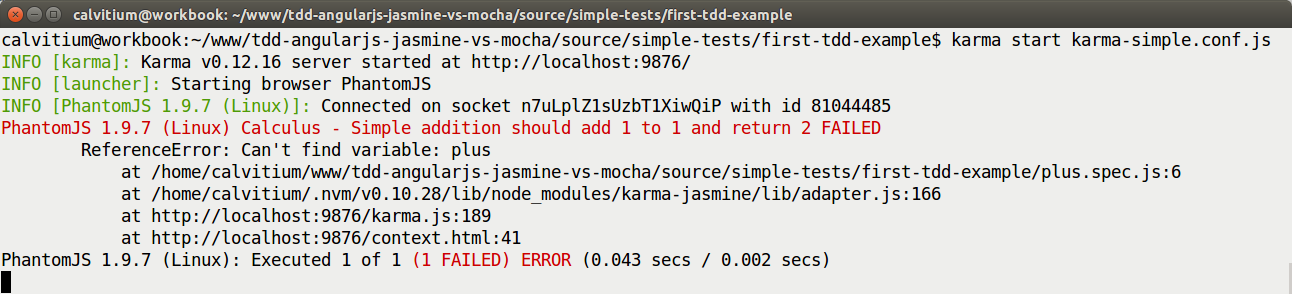
\includegraphics[width=12cm]{images/tdd-simple-step-1-1.png}
  }
  \caption{Terminal Ausgabe des ersten Tests}
  \label{figure:tdd-simple-step-1-1}
\end{figure}

Schritt 2: Zum Laufen bringen.
Um diesen Test möglichst schnell dazu zu bringen grünes Feedback zu geben, wird die einfachste und naiivste Implementierung verwendet.
Die einfachste Variante bedeutet also eine Funktion zu definieren, welche zwei Parameter übernimmt und \glqq{2\grqq} zurückgibt.

\begin{lstlisting}[style=verbo]
var plus = function(augend, addend) {
  return 2;
};
\end{lstlisting}

Wir wissen an dieser Stelle natürlich, dass hier eine klare, saubere und offensichtliche Lösung existiert. Es spricht natürlich nichts dagegen diese hier auch anzuwenden, um jedoch auch den dritten Schritt illustrieren zu können, wird hier naiv vorgegangen.\newline
Nach dieser naiven Implementierung ändert sich das Ergebnis des Tests von rot auf grün (siehe Abbildung \ref{figure:tdd-simple-step-1-2}).

\begin{figure}[H]
  \centering
  \fbox{
  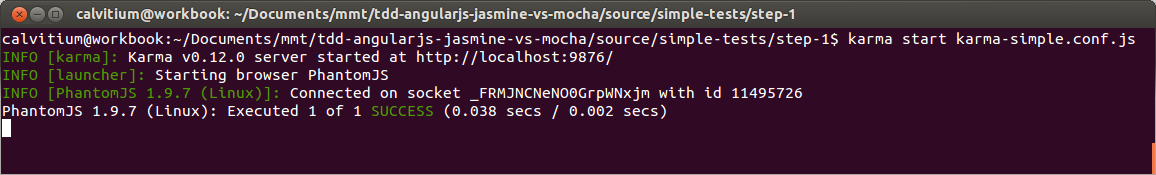
\includegraphics[width=12cm]{images/tdd-simple-step-1-2.png}
  }
  \caption{Terminal Ausgabe des ersten Tests nach naiver Implementierung}
  \label{figure:tdd-simple-step-1-2}
\end{figure}

Schritt 3: Es richtig machen.
Obwohl der Test nun bereits erfolgreich läuft, ist natürlich klar, dass diese naive Implementierung nicht korrekt ist. Es handelt sich um eine \glqq{Fake\grqq} Implementierung. Um nun die richtige Berechnung durchzuführen ändern wir die \glqq{plus(arg1, arg2)\grqq} Funktion folgendermaßen.

\begin{lstlisting}[style=verbo]
var plus = function(augend, addend) {
  return augend+addend;
};
\end{lstlisting}

Nach dem dritten Schritt wird erneut der Test ausgeführt um zu garantieren, dass das Korrigieren der naiven Implementierung auch funktioniert. Es wird ein positives Ergebnis erwartet (siehe Abbildung \ref{figure:tdd-simple-step-1-3}).

\begin{figure}[H]
  \centering
  \fbox{
  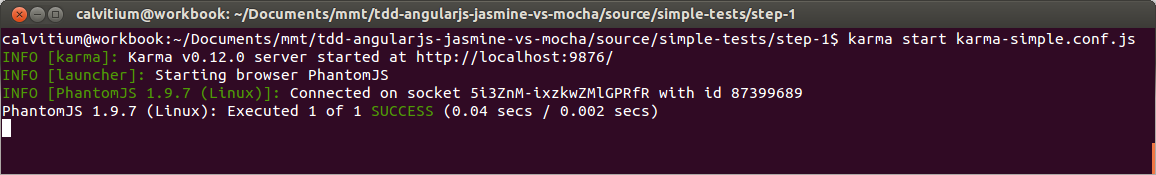
\includegraphics[width=12cm]{images/tdd-simple-step-1-3.png}
  }
  \caption{Terminal Ausgabe des ersten Tests nach Richtigstellung der Implementierung}
  \label{figure:tdd-simple-step-1-3}
\end{figure}

Durch die Anwendung des TDD-Kreislaufs wurde hier \textit{sauberer} und \textit{funktionierender} Code produziert.

% Wörter bis hier 1009 (36 Code)